\section{Qualitative Results}

\subsection{Sample Predictions}

Figure~\ref{fig:qualitative_preds} shows a selection of test tweets alongside the ground-truth label and predictions from all three models. Samples are grouped into three categories: (1) all three models correct, (2) mixed predictions, and (3) all three models wrong.

\begin{figure}[H]
    \centering
    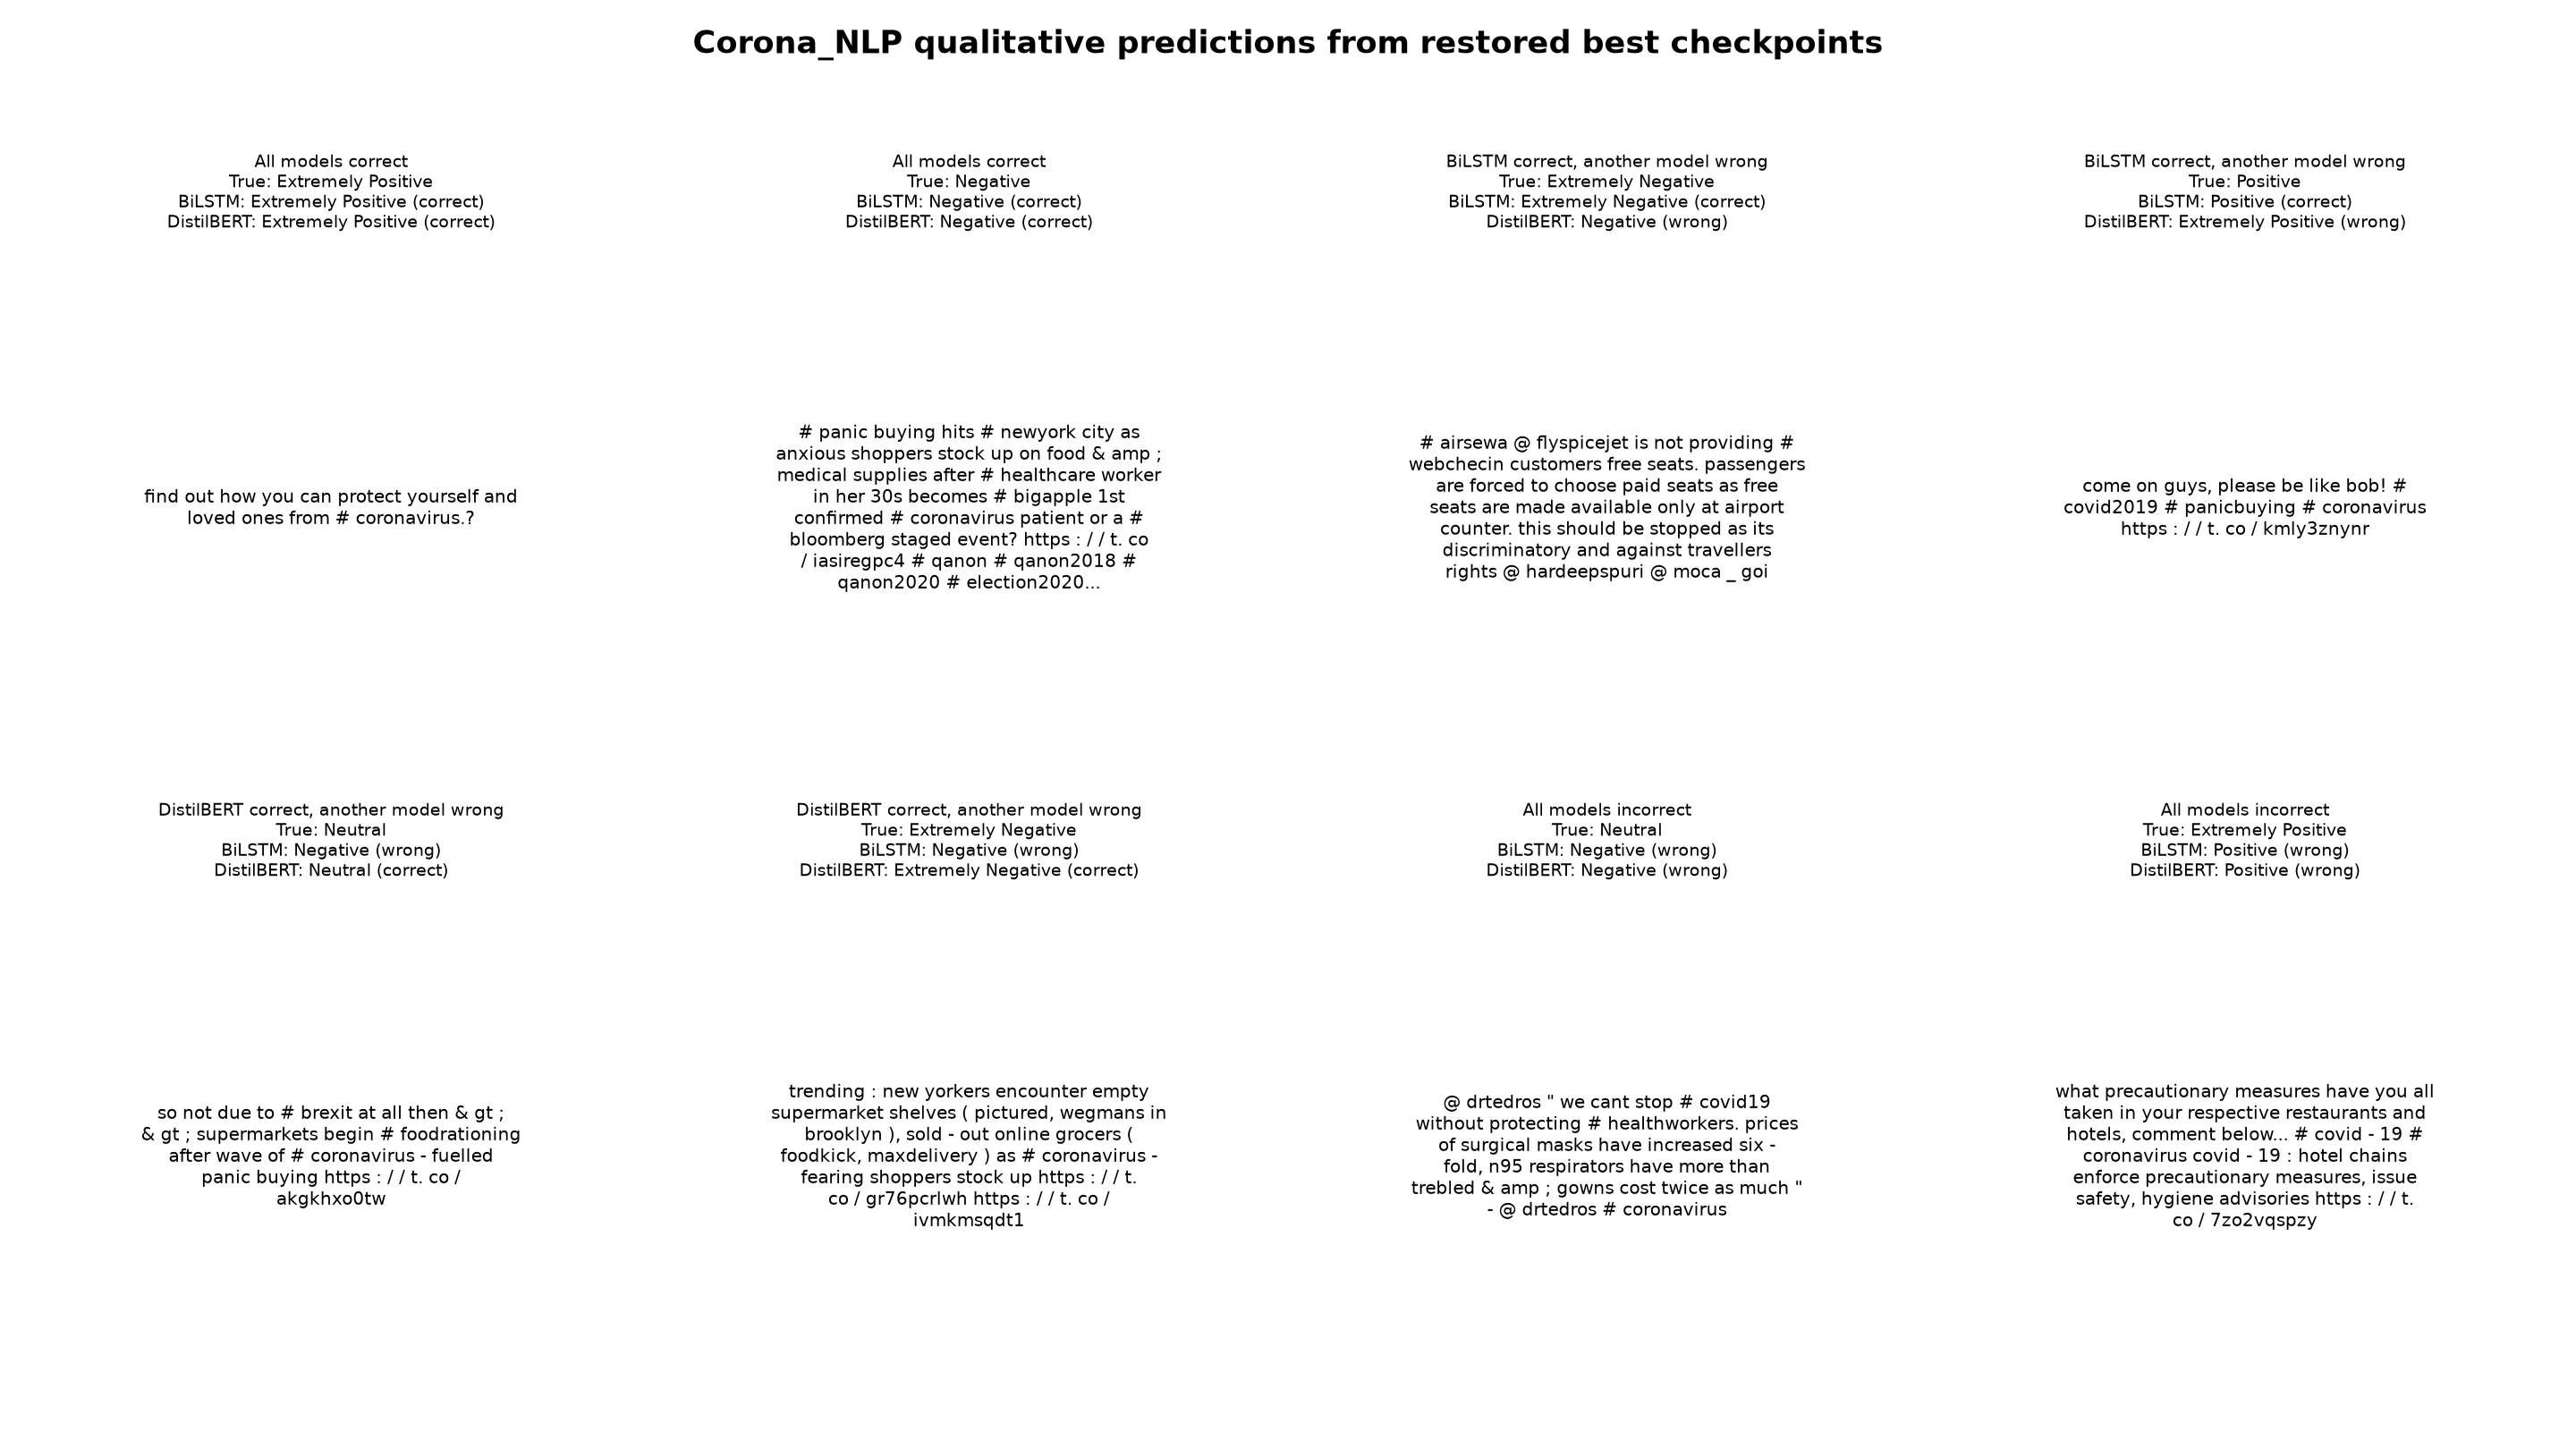
\includegraphics[width=\textwidth]{../../Assignment2/outputs/metrics/qualitative_predictions.png}
    \caption{Qualitative predictions on representative test tweets. Green cells indicate a correct prediction; red cells indicate an error. Each row shows the tweet text, the true label, and predictions from EXP-1, EXP-2, and EXP-3.}
    \label{fig:qualitative_preds}
\end{figure}

Inspection of the sample predictions reveals the following patterns:
\begin{itemize}
    \item \textbf{All-correct examples} tend to have clear, unambiguous emotional language (e.g.\ multiple positive exclamation marks or strongly negative disaster vocabulary). All three models handle these confidently.
    \item \textbf{Mixed examples} often involve subtle intensity distinctions (e.g.\ a tweet that is \textit{Negative} vs.\ \textit{Extremely Negative}). EXP-3 (full fine-tune) classifies these correctly more often than EXP-1, while EXP-2 (frozen) frequently collapses predictions to the nearest high-frequency class.
    \item \textbf{All-wrong examples} typically exhibit genuine label ambiguity: the tweet content could plausibly belong to two or more adjacent classes, suggesting annotation noise.
\end{itemize}

\subsection{Latent Space Visualisations}

Figures~\ref{fig:dimred_bilstm}, \ref{fig:dimred_frozen}, and~\ref{fig:dimred_full} show dimensionality-reduced visualisations (PCA, t-SNE, and UMAP) of the penultimate-layer representations for test-set samples, coloured by true sentiment class.

\begin{figure}[H]
    \centering
    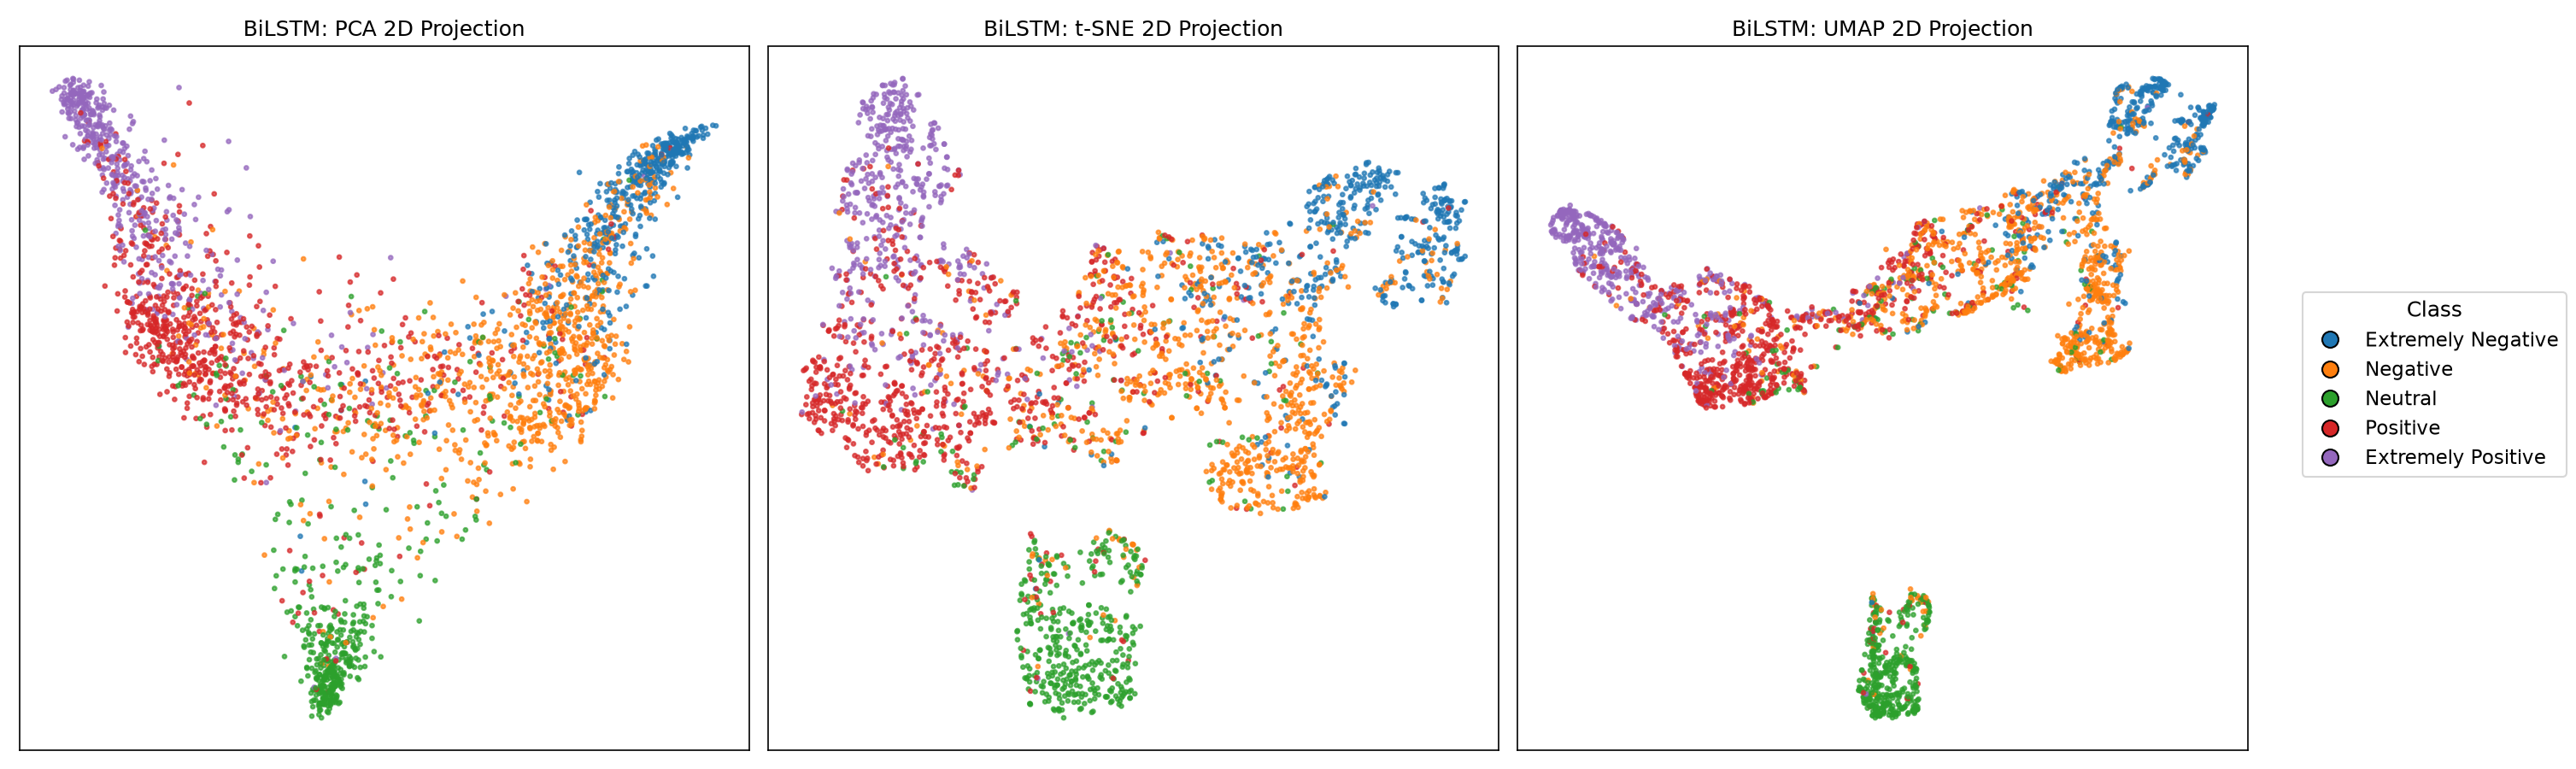
\includegraphics[width=\textwidth]{../../Assignment2/outputs/eda/bilstm_dimensionality_reduction.png}
    \caption{Dimensionality reduction of EXP-1 (BiLSTM) penultimate-layer representations on the test set. Each point is a tweet; colour denotes true sentiment class.}
    \label{fig:dimred_bilstm}
\end{figure}

\begin{figure}[H]
    \centering
    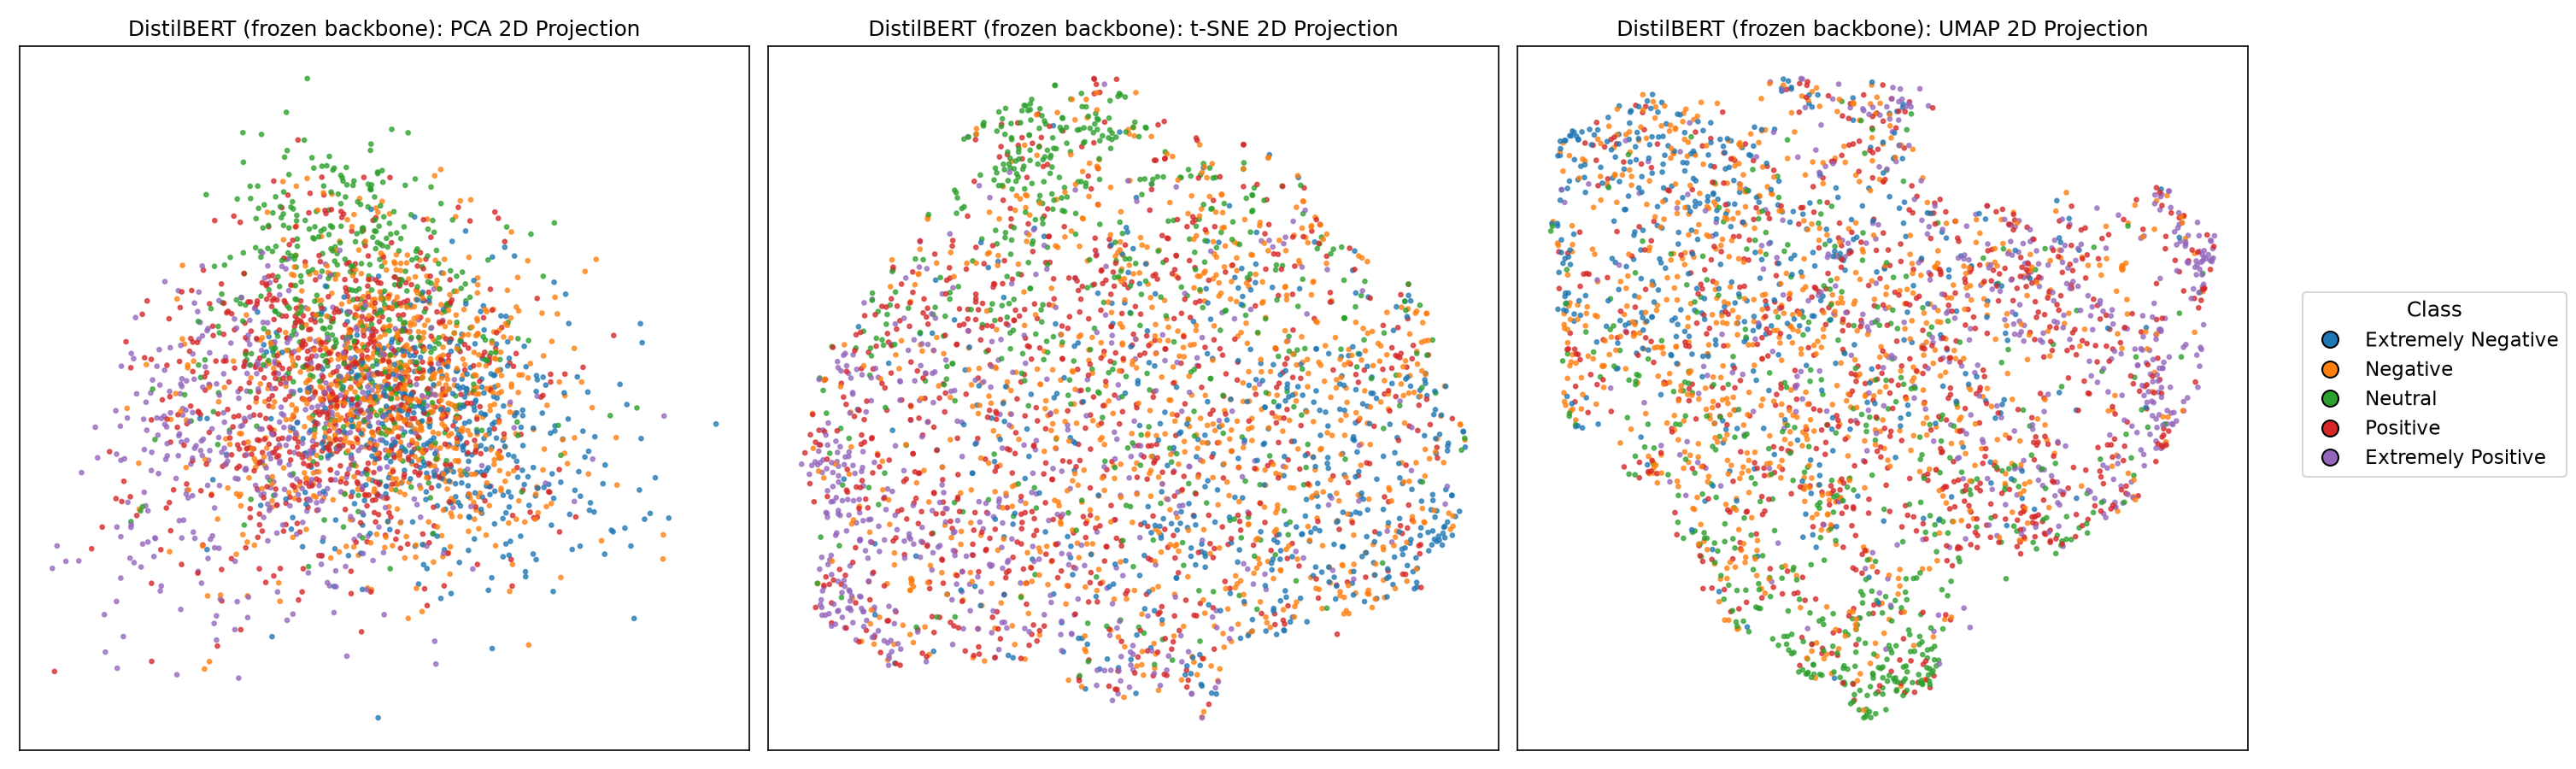
\includegraphics[width=\textwidth]{../../Assignment2/outputs/eda/distilbert (frozen backbone)_dimensionality_reduction.png}
    \caption{Dimensionality reduction of EXP-2 (DistilBERT frozen) \texttt{[CLS]} representations on the test set.}
    \label{fig:dimred_frozen}
\end{figure}

\begin{figure}[H]
    \centering
    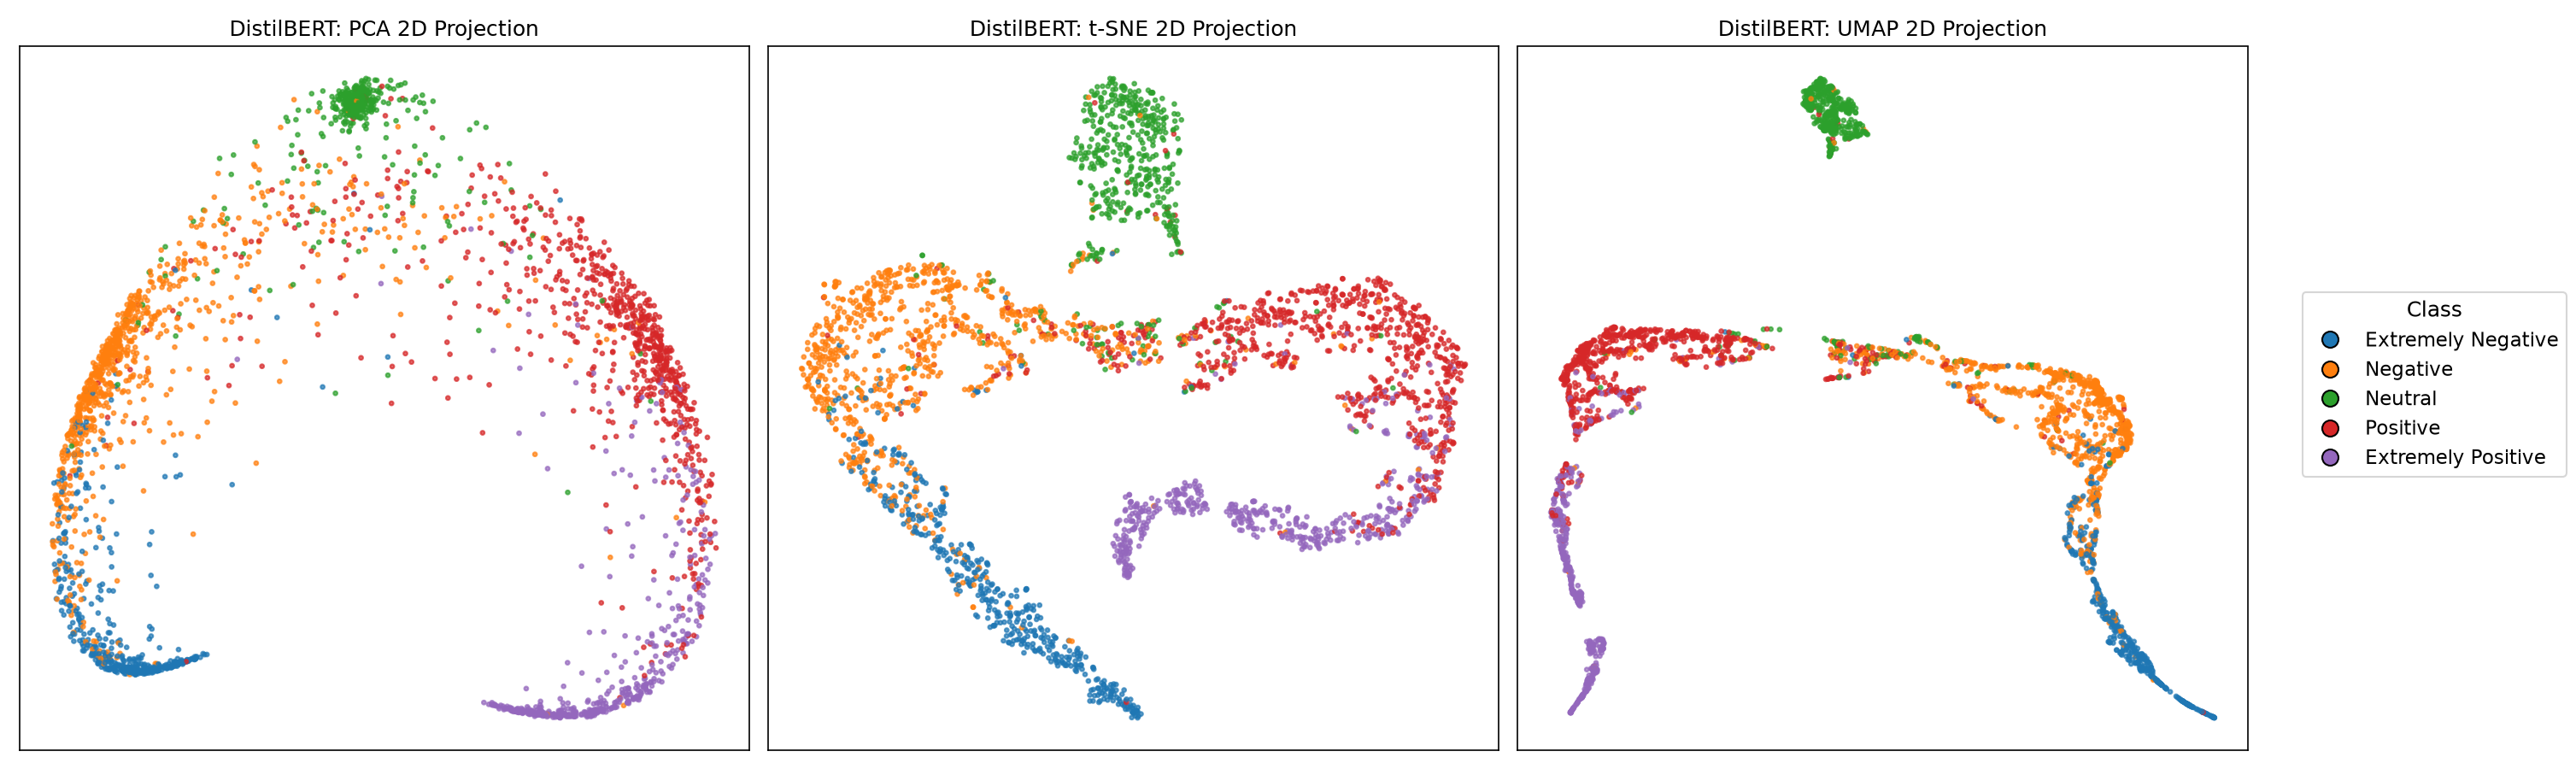
\includegraphics[width=\textwidth]{../../Assignment2/outputs/eda/distilbert_dimensionality_reduction.png}
    \caption{Dimensionality reduction of EXP-3 (DistilBERT full fine-tune) \texttt{[CLS]} representations on the test set. Classes are more linearly separable compared to EXP-1 and EXP-2.}
    \label{fig:dimred_full}
\end{figure}

Qualitative observations from the latent space plots:
\begin{itemize}
    \item \textbf{EXP-1 (BiLSTM):} Clusters are visible but overlapping, particularly for \textit{Negative}/\textit{Extremely Negative} and \textit{Positive}/\textit{Extremely Positive} pairs.
    \item \textbf{EXP-2 (Frozen):} Clusters are poorly separated, consistent with the low test accuracy. The frozen representations do not encode tweet sentiment in a linearly separable manner for a head trained only for 10 epochs.
    \item \textbf{EXP-3 (Full):} The five classes form visually distinct, well-separated clusters with minimal overlap, explaining the high test accuracy of 85.33\%.
\end{itemize}

\subsection{Class Similarity Matrices}

The class similarity matrix (cosine similarity between mean class-conditional representations) further illustrates the quality of the learned representations. For EXP-3, the \textit{Extremely Negative} and \textit{Extremely Positive} classes are most distinct from the central \textit{Neutral} class, while adjacent-intensity pairs (\textit{Negative}/\textit{Extremely Negative}; \textit{Positive}/\textit{Extremely Positive}) show higher mutual similarity — matching the expected ordinal structure of the sentiment scale.
